\documentclass{amsart}
\usepackage{graphicx}
\graphicspath{{./}}
\usepackage{hyperref}
\usepackage{csvsimple}
\usepackage{longtable}
\usepackage{lscape}
\usepackage{epigraph}
\title{Issues Fitting GHD To Q110}
\author{Zulfikar Moinuddin Ahmed}
\date{\today}
\begin{document}
\maketitle

\section{Manual GHD Fit of Q110}

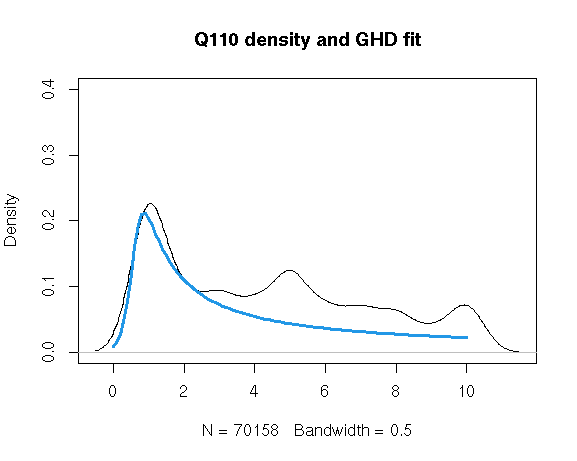
\includegraphics[scale=0.7]{handfitq110.jpeg}

GHD fits by MLE, but in some cases, we can fit manually, as above for Q110.  The parameters are a bit strange, which is what I worry about.

\begin{verbatim}
> caption<-paste(var, "density and GHD fit")
> out<-plot(density(V,bw=0.5),ylim=c(0,0.4),main=caption)
> xt<-seq(0,10,by=0.1)
> lines(xt,1.5*dghyp(xt,
object=ghyp(
lambda=0.1,
sigma=6,
mu=0.6,
gamma=90,
alpha.bar=0.04)),col=4,lwd=3)
> 
\end{verbatim}


\section{May 14 2021}

I look at the importance of Q110, on whether human race thinks hard work or luck determines success, and gain renewed enthusiasm for being more accurate in my models.

I take a step back from GHD and fit an exponential.

You see, when the substance is serious, we ought to respect the data and not be fooled by an automated technique, despite how it seems theoretically satisfying.  Nature comes first, not techniques.  One has to revere the data.

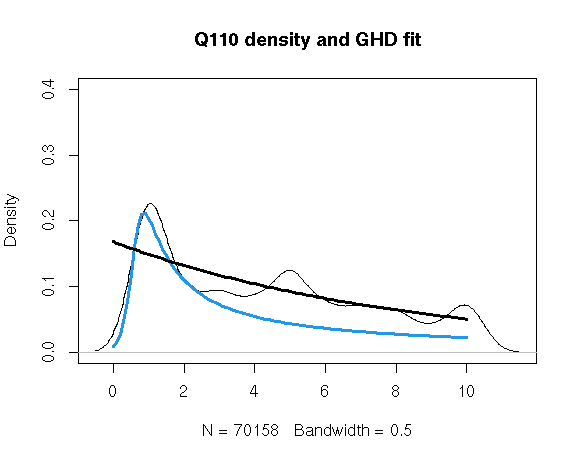
\includegraphics[scale=0.8]{fits-q110.jpeg}

The exponential fit is not all that bad at all.  Let's take a look at the summary.

\begin{verbatim}
> summary(mod)

Call:
lm(formula = log(nrm(Vt)) ~ t10)

Residuals:
     Min       1Q   Median       3Q      Max 
-0.48483 -0.25660 -0.08237  0.29677  0.59467 

Coefficients:
            Estimate Std. Error t value Pr(>|t|)    
(Intercept) -1.78406    0.27482  -6.492  0.00019 ***
t10         -0.11929    0.04429  -2.693  0.02736 *  
---
Signif. codes:  0 ‘***’ 0.001 ‘**’ 0.01 ‘*’ 0.05 ‘.’ 0.1 ‘ ’ 1

Residual standard error: 0.4023 on 8 degrees of freedom
Multiple R-squared:  0.4755,	Adjusted R-squared:   0.41 
F-statistic: 7.254 on 1 and 8 DF,  p-value: 0.02736
\end{verbatim}

Here we are getting an $R^2=0.41$ fit.  This is actually a good model. 

And this is how one develops a sense for the relative merits of the models.  Standard science takes over Zulf's thinking, after heady discovery and euphoria dies down and a different mode predominates. 

\end{document}]